% Created 2014-05-09 Fri 23:28
\documentclass[a4paper,6pt]{article}
\usepackage[utf8]{inputenc}
\usepackage[T1]{fontenc}
\usepackage{fixltx2e}
\usepackage{graphicx}
\usepackage{longtable}
\usepackage{float}
\usepackage{wrapfig}
\usepackage{rotating}
\usepackage[normalem]{ulem}
\usepackage{amsmath}
\usepackage{textcomp}
\usepackage{marvosym}
\usepackage{wasysym}
\usepackage{amssymb}
\usepackage{hyperref}
\tolerance=1000
\usepackage[margin=.75in]{geometry}
\usepackage[T1]{fontenc}
\usepackage[scaled=.7]{helvet}
\usepackage{courier} % tt
\linespread{1.01}
\author{N-CRITSER}
\date{\textit{<2014-05-06 Tue>}}
\title{267\_writeup.org}
\hypersetup{
  pdfkeywords={},
  pdfsubject={},
  pdfcreator={Emacs 23.4.1 (Org mode 8.2.4)}}
\begin{document}

\maketitle



\section{Abstract "TALK-A-LOT-BOT"}
\label{sec-1}
    My original goal for this project was to learn the underlying code for 
the Arduino platform while creating an anthropomorphic entity which "speaks"
and simulates eye movement while interacting with a user.  The general aspects
of this I have achieved, although I have adopted the usage of higher level 
libraries and forgone the learning of lower level aspects of the platform.  

    Currently the Talk-a-lot-Bot has as its central processing unit a Rev3 
Arduino Uno with an Ada-fruit Waveshield mounted to its I/O headers. The shield
controls the robots "voice".  Pre-recorded .WAV files are stored on a 
Fat 16 Formatted SD card.  This prerecording of all audio output does 
create a limitation on the flexibility of the Talk-a-lot-Bot.  But I strive 
to overcome this lack of natural randomness by introducing some irrationality
into the the output.  The wave files are chosen programmatically based on 
flags which are set as the running loop progresses.  Given a short amount of 
time the output could cycle but based on the flagging component it should not 
be an identical path through the wave file tree structure.  

    When a wave file is chosen it is played through the WaveHC library which
sends its wave file object through a low pass filter and opamp then to 
a stereo plug connector which sends the sound signal  to a speaker.  

Also, connected to the Uno, are 2 8x8 LED matrices, which are I2C protocol driven. 
The matrices cycle through various eye movements depending on the playing 
.WAV file.  All of this output can be manipulated (somewhat) by a button pad
with a 2 button option.  For most of the sound output the user is prompted by
the bot, to reply to some query.  Upon receiving an answer the bot responds,
not always in an intelligent manner.  In fact, It's my goal to give the bot
the sense of having some type of mental defect similar to Parry,
\url{http://en.wikipedia.org/wiki/PARRY}.   After, some testing I found that I had
more fun listening to Talk-a-lot, when he was being "Crazy" rather than 
attempting to interact in a prescribed "Boring" manner. 
\section{Components}
\label{sec-2}
\subsection{Adafruit waveshield sd card module}
\label{sec-2-1}
\subsection{Speaker}
\label{sec-2-2}
\subsection{Arduino Uno Rev3}
\label{sec-2-3}
\subsection{2-8x8 i2c led matrices for simulated eye movement}
\label{sec-2-4}
\subsection{adafruit libraries for graphics and sound}
\label{sec-2-5}
\section{Libraries}
\label{sec-3}
\begin{verbatim}
#include "Adafruit_LEDBackpack.h"

#include "Adafruit_GFX.h"
\end{verbatim}

\section{Wiring Diagram}
\label{sec-4}
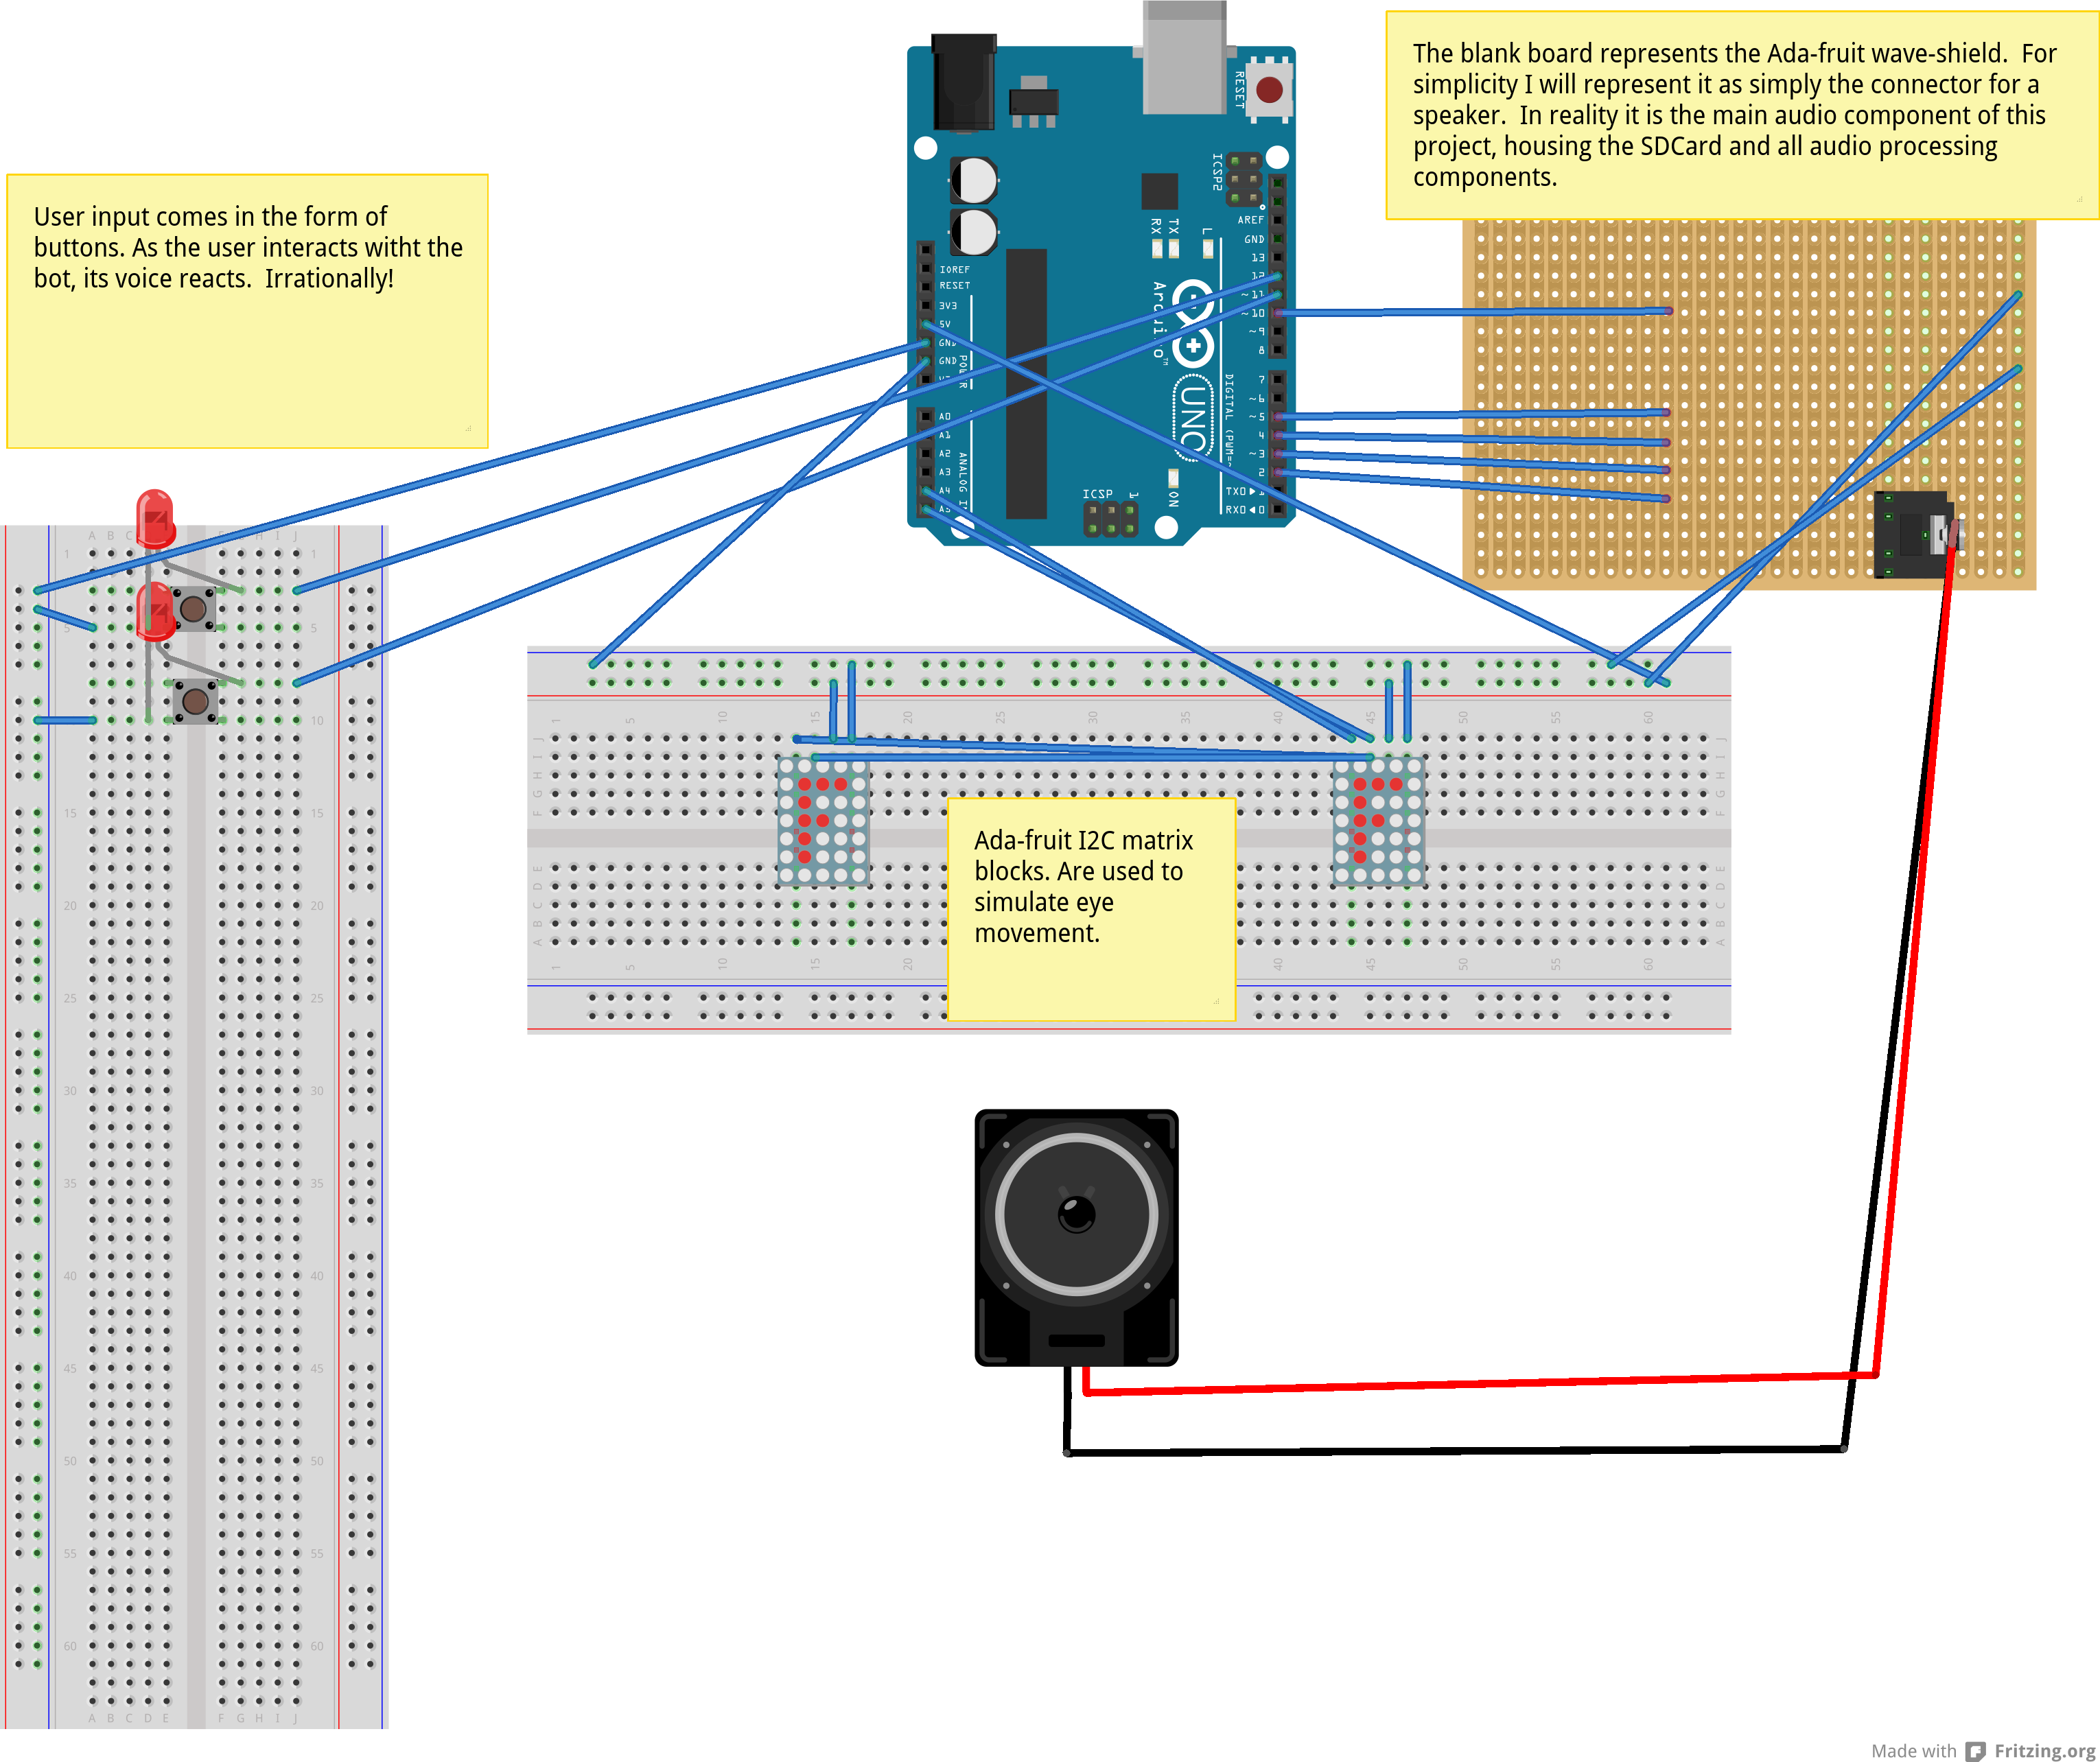
\includegraphics[angle=0,width=16cm]{./talk_a_lot_fritz_bb.png}
% Emacs 23.4.1 (Org mode 8.2.4)
\end{document}
